\marginnote{E\_Exp\_3}

This experiment mirrors Experiment 3, but focussing on instructions that did not use a number. 
We manipulated vagueness and the selection task (comparison and matching). 
In order to implement the experiment without mentioning numbers in the instructions, we changed the sequence of each trial to include a `target' (i.e., a dot array of a particular cardinality) before the instruction, so that we could then refer back to the target's cardinality in the instruction using expressions like \emph{the same number of dots as the target}; \emph{fewer dots than the target}.
This presentation of a target before the main body of the trial shares some features with \citeauthor[Experiment 2]{Izard20081221}, although in that experiment participants were told the cardinality of the target (called an \emph{inducer} in that paper) whereas in our experiment we did not tell participants the cardinality of the prime array.
An item was thus a combination of a target dot array, an instruction that did not contain a number, and a set of dot arrays taking their cardinalities from the same triples used in Experiment 2.
Table \ref{Instructions for e4} spells out how the instructions were constrained not to mention a numeral and gives examples of targets.

\begin{table}[htp]
\caption{Instructions and targets by condition for Experiment 4}
\begin{center}
\begin{tabular}{llcrl}
\hline\noalign{\smallskip}
Item					    &Selection task					& Vagueness	& Target		&Choose a square with\ldots							\\
\noalign{\smallskip}\hline\noalign{\smallskip}
\multirow{4}{*}{06:15:24} 	&\multirow{2}{*}{Comparison} 	& Crisp		& 20			&\ldots fewer dots than the target					\\
\cline{3-5}
							&								& Vague		& 20			&\ldots far fewer dots than the target				\\
\cline{2-5}
							&\multirow{2}{*}{Matching}		& Crisp		& 6			&\ldots the same number of dots as the target		    \\
\cline{3-5}
							& 		 						& Vague		& 10 		&\ldots about the same number of dots as the target	    \\
\noalign{\smallskip}\hline
\end{tabular}
\end{center}
\label{Instructions for e4}
\end{table}%
	
\subsection{Hypotheses}% E 4
\noindent For Experiment 4, we hypothesised:

\begin{description}
	\item [Hypothesis 1] Vague instructions are easier for the reader than crisp ones (main effect of vagueness)
	\item [Hypothesis 2] Comparison is easier for the reader than matching (main effect of selection)
	\item [Hypothesis 3] Effects of vagueness differ depending on whether selection is matching or comparison (interaction effect selection x vagueness, and focussed comparisons at each level of selection).
\end{description}

\subsection{Results}% E 4
40 volunteers participated.
The results showed that vagueness was beneficial for comparison but detrimental for matching (the same as Experiment 3) even when no numbers were allowed in the instructions. 
Figure \ref{resultse4} shows the means by condition. Our findings were as follows:

\begin{description}
	\item [Test of hypothesis 1] There was no significant main effect of vagueness ($\beta=-0.02$, $se=0.01$, $t=-1.5$, $p=0.1296$). 
	\item [Test of hypothesis 2] There was a main effect of selection, with comparison task instructions leading to faster responses than the matching task instructions ($\beta=0.18$, $se=0.02$, $t=10.4$, $p<0.0001$).  This effect was in the same direction as Experiment 3. 
	\item [Test of hypothesis 3] Vagueness did exert different effects depending on the selection task (main interaction effect of vagueness by selection $\beta=0.12$, $se=0.02$, $t=5.1$, $p<0.0001$). 
Separate analyses of the effect of vagueness were conducted for the comparison task and for the matching task using Bonferroni-adjusted significance thresholds. 
In the comparison task, vagueness resulted in faster response times ($\beta=-0.08$, $se=0.02$, $t=-4.3$, $p<0.0001$). 
In the matching task vagueness slowed response times ($\beta=0.05$, $se=0.01$, $t=3.7$, $p=0.0004$). 
These results are in the same direction as Experiment 3.
\end{description}

Once again, the cost reduction account was wrong to predict main effect advantages for vagueness, and wrong to predict that vagueness should be beneficial at each level of the selection task: however vagueness was advantageous in the comparison task.

\begin{figure}[htbp]
\centering
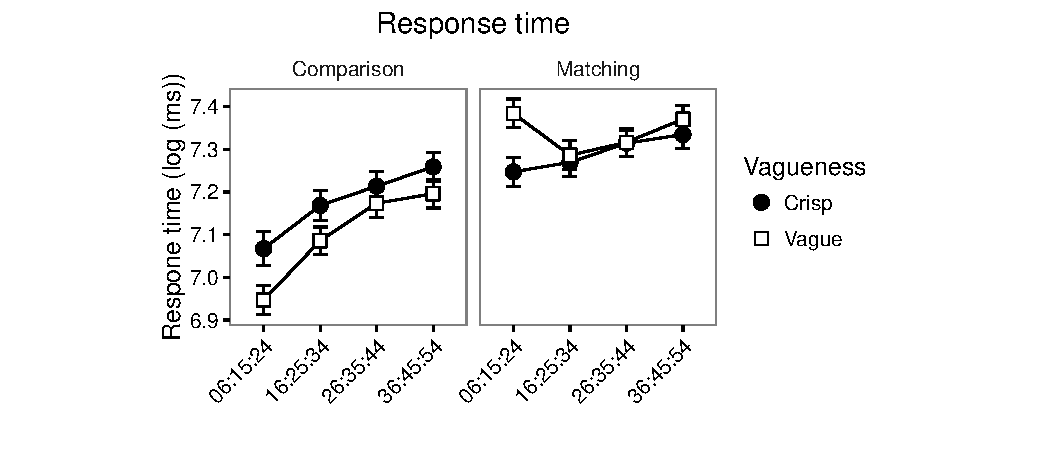
\includegraphics[width=\textwidth]{figures/e4-rtplot-1.pdf}
\caption{Mean response times by condition for Experiment 4}
\label{resultse4}
\end{figure}
